\section{Voice Recording}
This appendix describes the recording and subsequent manipulation of the sound used in the demonstration of the project results. The recording is in English. The speaker is a man with English as his second language. 

\subsection{Recording of speech}
\begin{table}[H]
	\centering
	\ra{1.3}
	\begin{tabular}{ c c c } \toprule
		{Item}	& {Description} 						& {AAU-no}. \\ \bottomrule 
		1	& Røde NT2000 	& aau14440-00	\\
		2	& Soundcard RME Fireface 802	& 86838 		\\
		3	& Computer running Matlab 2016a	 & 	NAN	\\
		\bottomrule
	\end{tabular}
	\caption{Table over equipment used for recording speech.}
	\label{tab:VoiceRec}
\end{table}
The recording of speech is performed in an anechoic chamber, where a male speaker is situated 1 m from the microphone. The used microphone is supplied with Phantom Power from the sound card. \\ 


\begin{figure}[H]
	\centering
	\tikzsetnextfilename{VoiceRecording}	
	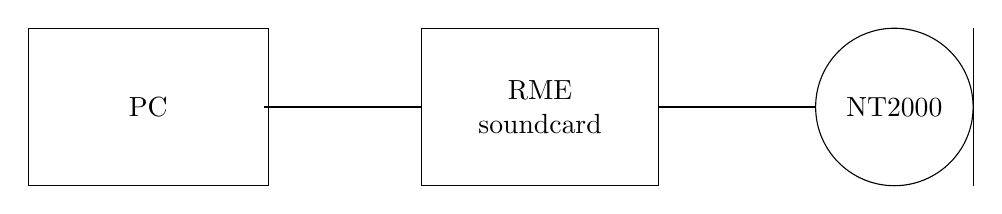
\begin{tikzpicture}
	\draw  (-2,1.5) rectangle (1.05,-0.5) node[pos=.5] {PC};
	\draw  (3,1.5) rectangle node[text width =1.75cm,text centered] {RME soundcard} (6,-0.5);
	\draw (1,0.5) -- (3,0.5);
	\draw  (9,0.5) ellipse (1 and 1)node[text width =1.75cm,text centered] {NT2000};
	\draw (10,1.5) -- (10,-0.5);
	\draw (8,0.5) -- (6,0.5);
	\end{tikzpicture}
	\caption{Voice recording setup.}
	\label{fig:VoiceRecording}
\end{figure}

The parameters chosen for the recording, prediction and cancellation are:
\begin{itemize}
	\item $N=1200$
	\item $O=1100$
	\item $M=1200$
	\item $P=10$
	\item Delay equal to $P=10$
	\item $f_s =48000$ Hz
	\item $\mu=0.001$
\end{itemize}


\subsection{The manuscript}
The manuscript is divided into sections, where different operations are made. Each section is stored in separate audio files for easier manipulation of the individual parts. 
 
\textbf{Normal voice}\\
\textit{This recording will demonstrate the performance of an Active Noise Control  system, in a headphone using Filtered-$x$ least mean squares combined with a linear prediction algorithm.} 

\textbf{Headphone filtered sound}\\
\textit{Now imagine that you have put on your headphones. I am speaking to you from the outside of the headphones.}

\textbf{FXLMS}\\
\textit{You have now activated the noise cancellation. This resembles the experience you would get from a noise canceling headphone, when a person is speaking from outside of the headphone. 
Here no prediction was used. Now the predictor is activated. }

\textbf{LP FXLMS}\\
\textit{This is the filtered-$x$ least means squares combined with the linear prediction algorithm. This should be almost inaudible to you. We will now listen to the predictor on its own.}

\textbf{The predicted sound}\\
\textit{In case you didn't hear what I just said, you are now listening to the predictor predicting 25 $m$s ahead in time. You are listening to an estimate of what I am going to say.}

\textbf{Summary}\\
We hope you enjoyed the demonstration. Thank you for listening.\\\\

The sections in the manuscript are filtered in the following way:
\begin{table}[H]
	\centering
	\ra{1.3}
	\begin{tabular}{ c c } \toprule
		{Section}				& {Manipulation} \\ \bottomrule 
		Normal Voice			& No manipulation  	\\
		Headphone filtered sound& Filtered with Headphone transfer function \\
		FXLMS					& Filtered with FXLMS	\\
		LP FXLMS 				& The output of the proposed algorithm	\\
		The predicted signal 	& The output of the predictor	\\
		Summary 				& No manipulation	\\
		\bottomrule
	\end{tabular}
	\caption{Manipulation of the different parts of the recording.}
	\label{tab:VoiceRecSections}
\end{table}

The recordings are available here: \\
\url{https://www.youtube.com/watch?v=aSd2qz_pUPA} 













